%%%%%%%%%%%%%%%%%%%%%%%%%%%%%%%%%%%%%%%%%%%%%%%%%%%%%%%%%%%%%%%%%%%%%%%%%
%                                                                      	%
%     File: Thesis_I2C.tex                          				 	%
%     Tex Master: Thesis.tex                                			%
%                                                                      	%
%     Author: Carlos A. Rodrigues                         				%
%     Last modified : 15 Abril 2013                         			%
%                                                                      	%
%%%%%%%%%%%%%%%%%%%%%%%%%%%%%%%%%%%%%%%%%%%%%%%%%%%%%%%%%%%%%%%%%%%%%%%%%

\chapter{I2C}
\label{chapter:i2c}


Explicar o protocolo i2c. como funciona e as linhas que tem. explicar em que acasos é mais usado


O \acrshort{soc} utilizam uma memoria de pequenas dimensões, não voatil, que permita guardar alguns dados em caso de algum problema com o \acrshort{soc}, como falta de energia. Permitindo assim que o \acrshort{soc} saiba que horas eram quando faltou a energia. Estas memorias utilizam para comunicar com o \acrshort{soc} o barramento de \acrshort{i2c}. Éste barramento utiliza apenas duas linhas para comunicação, como é um barramento síncrono uma das linas é o sinal clock \acrshort{scl}, a outra linha \acrshort{sda} é utilizada para transferência de dados entre o mestre e o periférico. Apesar de ser um barramento relativamente lendo, comparado com o \ref{chapter:spi}, de transferência de dados, é um barramento bastante utilizado pela sua simplicidades de adicionar mais periféricos aos já existentes, como se pode ver na figura \ref{fig:licacoesI2C}, para adicionar um periférico é necessário apenas ligar as duas linhas do barramento ao periféricos. Em vez de utiliza uma linha para selecionar o periférico com que quer comunicar como no \ref{chapter:spi}, todos os periféricos tem o seu endereço de sete bits, em alguns periféricos permitem a alteração dos bits menos significativos. Como se pode ver na Figura XXXX o mestre envia um endereço de oito bits, sendo os sete bits mais significativos os que definem o escravo e o bit menos significativo é utilizado pelo mestre para informar ao escravo se pretende escrever, com o bit a zero, ou ler, com o bit a 1. Como existem apenas duas linhas de comunicação o barramento utiliza vários sinais interpretado pelos escravo e pelo mestre para poderem comunicar entre si, mais a frente no subcapítulo \ref{i2c_diagrama} serão explicados os vários sinais existentes. Cada operação começa com um sinal de start bit \ref{i2c_start} seguido de 8 bits correspondente ao endereço do escravo que se pretende comunicar, com a informar se é uma leitura ou uma escrita. De seguida o escravo responde com um ACK \ref{i2c_ack}. No caso de ser uma leitura em seguida o escravo envia os dados para o mestes e este responde com um ACK \ref{i2c_ack},  este processo do escravo enviar dados e o mestre enviar ACK \ref{i2c_ack} é repetido continuamente até o mestre ter os dados necessários e responder com um NACK \ref{i2c_nack} seguido de um sinal de \ref{i2c_stop}. No caso de ser um escrita a diferença para o anterior é quem envia os dados e os ACK \ref{i2c_ack}, passado o mestre a enviar os dados e os escravo e enviar os ACK \ref{i2c_ack}, e quando mestre já tiver enviado os dados todos este em vez de enviar dados envia um sinal de Stop \ref{i2c_stop}, este processo pode se visto de maneira sucinta na figura XXXX.


por figura com o protocolo dos endereços


\begin{figure}[!htb]
  \centering
  \includegraphics[width=0.50\textwidth]{Figures/I2C.png}
  \caption[Protocolo I2C]{Esquematico do sistema de comunicação I2C, com 1 master e vários escravos"tirou do wiki".}
  \label{fig:ligacoesI2C}
\end{figure}


\section{Mestre I2C}

A openRisc tem disponivel um core \acrshort{i2c} mestre com uma ligação Wishbone para se ligar se ligar ao processdor do \acrshort{soc}. Apesar deste cores estar em desenvolvimento ainda  não estava a trabalhar correctamente, tanto na leitura como na escrita de dados no escravo. A utilização deste barramento tem como objectivo poder guardar dados caso seja existe alguma problema com o \acrshort{soc}, por isso é necessário que este trabalhe correctamente na leitura como na escrita de dados.

O core mestre \acrshort{i2c} está subdividido por várias camadas, como se pode ver na figura \ref{fig:fluxo_I2C_master}. O barramento Wishbone comunica directamente com a camada Master I2C top, que faz toda a gestão do protocolo \acrshort{i2c} com o barramento Wishbone de entrada e saida de dados do core. Caso se pretenda efetuar uma escrita para o escravo o Master I2C top excita o I2C Byte e envia a palavra de 8 bits que se pretende enviar para o escravo. Neste nível da camada a palavra é subdividida e envida para a ultima camada I2C bit conforme esta for solicitando. Nesta ultima camada é gerada a onda de clock ao mesmo tempo que é enviado o bit para a linha de dados \acrlong{sda}. No barramento \acrshort{i2c} ao contrario do barramento \ref{chapter:spi} não é possível efetuar uma leitura e escrita simultaneamente. Por isso corresponde a uma processo novo quando se pretende fazer uma leitura, começando por haver uma troca de informação entre camadas , da mais alta para a mais baixa, a indicar que se pretende fazer uma leitura. Quando a camada mais baixa recebe essas informação ela começa a gerar cloks que são recebidos pelo escravo, e este envia os dados que tem para enviar. Em simultâneo a camada I2C Byte fica em estado de prontidão a espera que a camada mais baixa I2C bit lhe envie um bit para ser guardado numa palavra de 8 bits. Quando são recebidos os 8 bits de dados do escravo a palavra é enviada para a camada mais alta Master I2C top, que por sua vez envia para o processador pelo barramento Wishbone.

\begin{figure}[!htb]
  \centering
  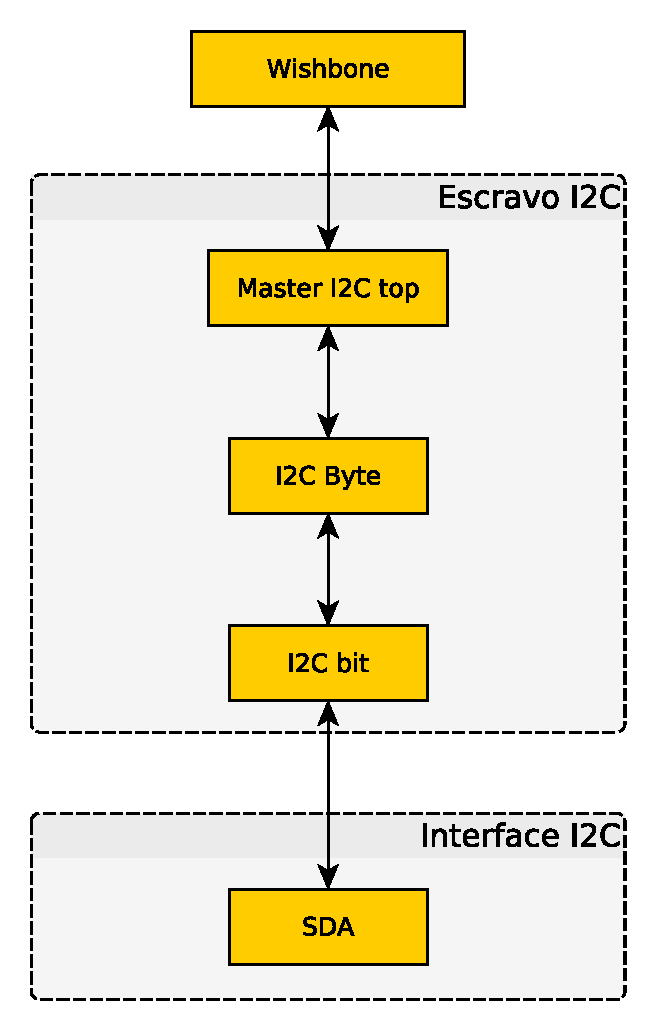
\includegraphics[width=0.50\textwidth]{grafos/diagrama_I2C_master.pdf}
  \caption[Fluxo de dados do core mastre I2C]{Fluxo de dados do core master I2C}
  \label{fig:fluxo_I2C_master}
\end{figure}

O mestre \acrshort{i2c} tem disponivel dois barramentos os Wishbone para transmitir dados para o processador e o barramento \acrshort{i2c} para comunicação com os escravos. Todos os sinais estão descritos na tabela \ref{table:sinais_I2C_master}. Como pode ver na tabela a parte do barramento \acrshort{i2c} tem 3 vezes mais sinais que o barramento de \acrshort{i2c} explicado anteriormente. Isto deve-se ao por o core não ser tri-state ou seja não tem três estado, o estado 1, 0 e alta indução, então essa gestão é feita fora de cada core. Sendo as linhas de comunicação entre os dois cores o scl\_pad\_i é o sinal de clock e sda\_pad\_i para a transmissão de dados. 

por a tabela de sinais da interface de i2c (sinais de entrada e saida)
\begin{table}[h!]
  \begin{center}
    \begin{tabular}{|C{2cm}|c|c|c|}
      \hline
      Interface & Nome & direcção & Descrição \\
      \hline \hline
      \multirow{10}{*}{Wishbone} & wb\_clk\_i & input & Clock, Recebido pelo Wishbone. \\
      \cline{2-4}
      & wb\_rst\_i & input & Reset, renicia o core quando se encontra no valor logico "1".\\
      \cline{2-4}
      & arst\_i & input & Reset assincrono, renicia o core quando se encontra no valor logico "1".\\
      \cline{2-4}
      & wb\_adr\_i & input & Endereço do registo onde se pretende ler ou escrever no core.\\
      \cline{2-4}
      & wb\_dat\_i & input & Recepecção de dados por parte do processador.\\
      \cline{2-4}
      & wb\_dat\_o & output & Envio de dados para o processador.\\
      \cline{2-4}
      & wb\_we\_i & input & Bit de selecção de escrita.\\
      \cline{2-4}
      & wb\_stb\_i & input & \\
      \cline{2-4}
      & wb\_cyc\_i & input & \\
      \cline{2-4}
      & wb\_ack\_o & output & bit que informaça o processador a recepecção do comando pelo core.\\
      \cline{2-4}
      & wb\_inta\_o & output & bit de interrupção. \\
      \hline \hline
      \multirow{6}{*}{I2C} & scl\_pad\_i & input & sinal de clock\\
      \cline{2-4}
      & scl\_pad\_o & output & sinal de clock .\\
      \cline{2-4}
      & scl\_padoen\_o & output & habilitador do sinal de clock .\\
      \cline{2-4}
      & sda\_pad\_i & input & sinal de dados\\
      \cline{2-4}
      & sda\_pad\_o & output & sinal de dados .\\
      \cline{2-4}
      & sda\_padoen\_o & output & habilitador do sinal de dados .\\
      \hline
    \end{tabular}
  \end{center}
  \caption[Tabela de sinais do core I2C master]{Tabela de sinais da interface I2C master}
  \label{table:sinais_I2C_master}
\end{table}

Na gestão do barramento tri-state é feito foi duas linhas para cada sinal no caso do clock temos o sinal scl\_pad\_o, que não é mais que um sinal que tem sempre o valor lógico '0'. O outro sinal é o scl\_padoen\_o este sinal vai variando conforme como um clock comutando o sinal de clock scl\_pad\_i entre o valor lógico '0' e o valor de alta impedância. Aparentemente o sinal de clock estaria a varias entre o valor lógico '0' e o de alta impedância que não corresponde a nenhum estado logico possível de determinar. Mas o sinal de clock encontra-se ligado por uma resistência a uma tensão igual ao valor lógico '1', como pode ver na figura XXXXXX. Então sempre que se encontrar no estado de alta impedância é como se tivesse no valor lógico '1', mas permitindo que ambos os cores coloquem o valor lógico '0' sempre que pretendam, bastando por o sinal de clock a '0'. A lógica para o sinal de dados é igual ao de sinal de clock sendo o sinal sda\_pad\_o o que se encontra sempre no valor lógico '0' e o sinal sda\_padoen\_o vai variando conforme a informação que necessita enviar.

por uma imagens para explicar o tri-state XXXXXX

Na tabela \ref{table:registos_I2C_master} podemos ver os registos existentes no mestre \acrshort{i2c}. Estes registos são utilizados para configurar o core mestre, como configurar a frequência de clock, ver o estado do core da reseccao e da transmição dos dadospara o core escravo. 

tabela de registos (endere\c{c}os do registos).
\begin{table}[h!]
  \begin{center}
    \begin{tabular}{|c|c|C{8cm}|c|}
      \hline
      Nome & leitura/escrita & Descrição & Offset End. \\
      \hline \hline
      Ajuste do clock & escrita e leitura & ajuste da frequência de clock 8bits menos significativos  & 0X00 \\
      \hline
      Ajuste do clock & escrita e leitura & ajuste da frequência de clock 8bits mais significativos  & 0X01 \\
      \hline
      Registo de controlo & escrita e leitura & disponibiliza várias informações do estado do core & 0X02 \\
      \hline
      Leitura de dados & leitura & leitura dos dados recebidos pelo I2C & 0X03 \\
      \hline
      Escrita de dados & escrita & escrita dos dados a enviar pelo I2C & 0X03 \\
      \hline
      Registo de estado & leitura & indica o estado do core & 0X04 \\
      \hline
      Registo de Debug & leitura & envio o que foi escrito pelo processador para o core.& 0X05 \\
      \hline
      Registo de estado & leitura & indica o estado do core, que comando se encontra a realizar. & 0X06 \\
      \hline
      Endereço do escravo & escrita e leitura & endereço do escravo onde que se encontra a escrever ou a ler.  & 0X07 \\
      \hline
    \end{tabular}
  \end{center}
  \caption[Tabela de registo do core I2C master]{Tabela de registos da interface I2C master}
  \label{table:registos_I2C_master}
\end{table}

O core mestre de \acrshort{i2c} tem disponível o processo de leitura e escrita. No processo de escrita do mestre é necessário configurar o mestre antes, com a informação da frequência do sinal de clock do protocolo \acrshort{i2c}. apos a configuração é necessário enviar para o mestre o endereço do escravo que pretendemos comunicar, este endereço já vem com o bit menos significativo com o valor logico 1 ou 0 conforme pretendemos escrever ou ler do escravo como foi explicado anteriormente. Por fim efetuamos uma leitura ou escrita ao endereço de Offset 0X03 o core mestre que irá enviar os dados recebidos para o escravo ou irá pedidos os dados ao escravo e erá enviar para o processador.  

\section{escravo I2C}

A comunidade OpenRISC ainda não tinha desenvolvido nenhum core \acrshort{i2c} escravo. No processo do seu desenvolvimento constantei que o core \acrshort{i2c} mestre sem a parte que faz a gestão do barramento Wishbone, e com uma nova camada de alto nível que realizasse a gestão com uma memoria ou com outro tipo de periférico com wishbone, teríamos um core de \acrshort{i2c} escravo. na construção desde cores foi utilizado as duas camadas mais baixas do mestres, ou seja os ficheiros I2C bit e o I2C byte. Para o funcionamento foi preciso criar uma maquina de estados no nivel mais alto, que efectua o controlo entre o protocolo I2C e a memoria, como se pode ver na figura \ref{fig:fluxo_I2C_slave}. O Fluxo de informação no core começa pelo pela camada mais baixa ou seja no I2C bit que recebe do sinal \acrshort{sda} e envia para a camada superior I2C byte onde agrupo os bits em palavras de 8 bits e envia para a maquina de estado onde está conforme o estado que esteja envia para a memoria essa informação para ser guardada do endereço definido, isto no caso que se esteja a efectuar uma escrita. No caso de uma leitura a maquina de estado recebe o endereço de leitura realiza uma leitura a memoria e envia para o I2C byte, onde vai separar a palavra de 8 bits por bits e vai ser sendo enviado conforme este for pedindo pelo I2C bit que vai enviado para o I2C mestre.  

por uma imagem que mostra que tirei o codigo do mestre e criei o escravo.

\begin{figure}[!htb]
  \centering
  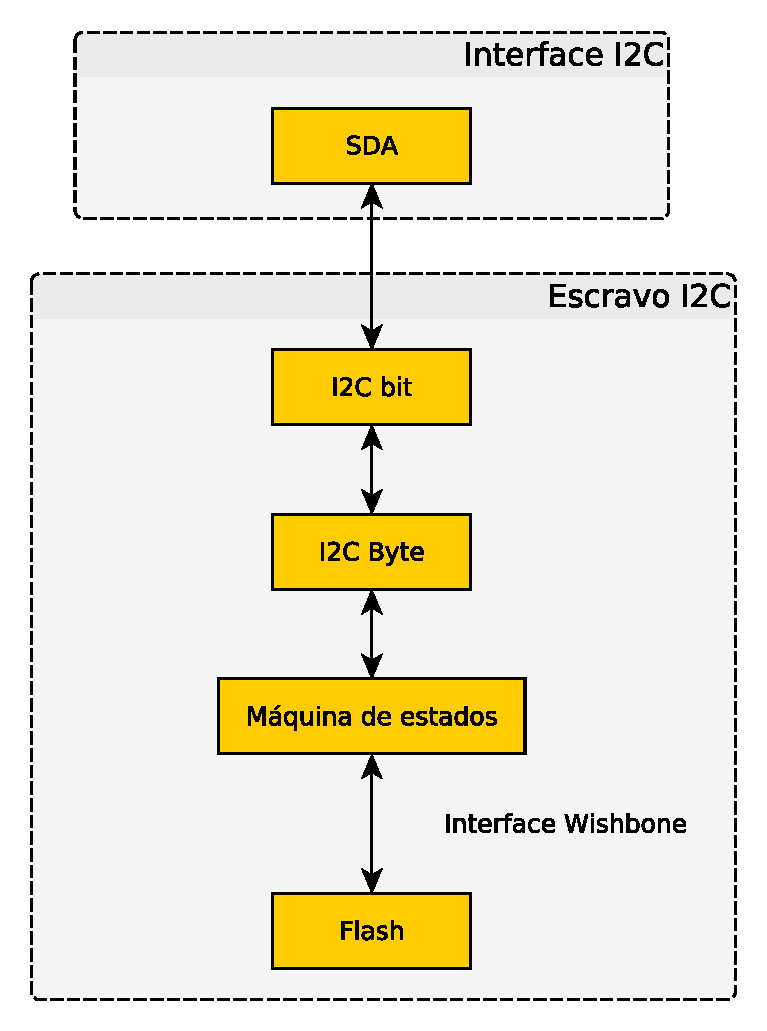
\includegraphics[width=0.50\textwidth]{grafos/diagrama_I2C_slave.pdf}
  \caption[Fluxo de dados do core escravo I2C]{Fluxo de dados do core escravo I2C}
  \label{fig:fluxo_I2C_slave}
\end{figure}

Na tabela \ref{table:slave} tem uma breve descrição das ligações que o escravo tem disponível. O escravo conta com um conjunto de ligação de I2C iguais ao do mestre para controlar o as duas linhas da ligação de I2C. Para alem dessas ligaçoes conta com um sinal de Clock que é gerado pelo sistema, um sinal de reset que é utilizado para por as definições default do core e um sinal de interrupção que é utilizado se for pretendido receber informação do core, como por exemplo de algo correu mal do processo que está a decorrer.

\begin{table}[h!]
  \begin{center}
    \begin{tabular}{|c|c|c|}
      \hline
      Nome & direcção & Descrição \\
      \hline \hline
      clk\_i & input & Clock, Recebido do sistema. \\
      \hline
      rst\_i & input & Reset, renicia o core quando se encontra no valor logic "1".\\
      \hline
      scl\_i & input & sinal de clock\\
      \hline
      scl\_padoen\_o & output & habilitador do sinal de clock .\\
      \hline
      scl\_pad\_o & output & sinal de clock .\\
      \hline
      sda\_i & input & sinal de dados\\
      \hline
      sda\_padoen\_o & output & habilitador do sinal de dados .\\
      \hline
      sda\_pad\_o & output & sinal de dados .\\
      \hline
      irq\_o & output & interrupcção .\\
      \hline
    \end{tabular}
  \end{center}
  \caption[Tabela de sinais do core I2C slave]{Tabela de sinais da interface I2C slave}
  \label{table:slave}
\end{table}

O modo de funcionamento do core escravo de I2C, inicialmente permanece a escuta na linha dos dados e ficando a espera do Start bit. quando assim acontece o core fica a espera de receber o meu endereço enviado pelo mestre. Quando é recebido o seu endereço o escravo identifica pelo ultimo bit se o mestre pretende efetuar uma leitura ou uma escrita. Conforme esse precessão o escreve evolui para o estado correspondente dentro da maquina de estados interna. De seguida o mestre envia o 3 conjuntos de 8 bits que é o endereço onde se vai efetuar a escrita ou a leitura. No caso de uma escrita, o escravo fica a espera que o mestre gere sinais de clock efetua leitura na linha de dados quando tiver recebido os 8 bits da palavra responde com um ACK. Como este core escravo é uma memoria grava essa palavra no endereço da memoria especificado pelo mestre, e incrementa uma posição ao endereço. voltando a ficar a escuta de novos dados por parte do mestre, até que mestre envie o stop bit depois do escravo o ter enviado. No caso de ser de leitura depois de receber o endereço onde que o mestre pretende ler, efectua uma leitura a posição de memoria, e incrementa uma posição ao endereço de memoria. Ficando a espera que o mestre gere sinais de clock para poder a palavra lida da memoria, depois de enviar voltar ler e volta a ficar a espera que o mestre gere o sinal de clock. Até que o mestre responda com NACK e de seguinda envie um Stop Bit. O escravo responde ao mestre a todas as palavras recebidas com um ACK.


\section{diagrama temporal}
\label{i2c_diagrama}
o protocomo de comunicação de I2C usa várias combinações temporais permitindo um intendimento entre o mestre e os vários escravos existentes no barramento de comunicação. resumindo a explicação feita anteriormente do protocolo de comunicação, qualquer comunicação entre os dois cores começa com o \ref{i2c_start} e é finalizado sempre com um \ref{i2c_stop}. Sempre que um core recebe oito bits tem de enviar um \ref{i2c_ack}, o \ref{i2c_nack} é enviado automaticamente caso o cores não responda com o com o ACK. Visto que a linha de dados tem o valor logico '1' caso ninguém o force ao valor logico '0' como foi explicado anteriormente.

\subsection{Start bit}
\label{i2c_start}
O sinal Star bit utilizado desperta os cores escravos que vai começar a ser enviado um dados. O sinal de dados quando se encontras no valor de alta impedância o mestre força o valor lógico de '1' quando a onda de clock está no lado negativo da onda. Quando o clock está no lado positivo da onda o mestre força os dados a '0', até que o clock volte a estar no lado negativo da onda, como se pode ver na figura \ref{fig:Start_I2C}. 

 \begin{figure}[!htb]
   \centering
   \includegraphics[width=0.50\textwidth]{ondas/I2C_S.pdf}
   \caption[Bit de inicialização]{Bit de inicialização}
   \label{fig:Start_I2C}
 \end{figure}

\subsection{Stop bit}
O sinal Stop bit que informa o core escravo que toda a informação pretendida já foi enviada ou recebida. Quando a onda de clock se encontra no lado negativo o mestre forca o estado a onda de dados no valor lógico '0', quando o clock passa para o lado positivo da onda o mestre escreve no sinal de dados o valor lógico de '1'. ficando neste estado até que o sinal de clock esteja no lado negativo da onda. esta onda pdoe ser vista de força simplificada na figura \ref{fig:Stop_I2C}.
\label{i2c_stop}
 \begin{figure}[!htb]
   \centering
   \includegraphics[width=0.50\textwidth]{ondas/I2C_ST.pdf}
   \caption[Bit de paragem]{Bit de paragem}
   \label{fig:Stop_I2C}
 \end{figure}

\subsection{Restart bit}
O sinal de restart bit não passa de um conjunto dos dois sinais anteriores, um sinal de stop bit seguido de um sinal de start bit, como se pode perceber na figura \ref{fig:Restart_I2C}.
 \begin{figure}[!htb]
   \centering
   \includegraphics[width=0.75\textwidth]{ondas/I2C_R.pdf} %0.5
   \caption[Bit de recomeço]{Bit de recomeço}
   \label{fig:Restart_I2C}
 \end{figure}

\subsection{Dados}
Depois de se pode iniciar e parar uma comunicação é importante saber transmitir dados. Nos próximos dois capitulos temos uma breve explicação de como é transmitido um bit com um valor '1' e valor '0'. Quando se envia um bit, esse dados mantem-se no sinal de dados durante um ciclo de clock completo e se for necessario o valor do sinal dos dados é alterado quando o sinla de clock se encontra com o valor negativo.

\subsubsection{Valor logico '1'}
O core que quer enviar o bit com o valor 1 forca o sinal de dados ao valor lógico 1 quando o clock tem o valor negativo. Mantem esse valor durante um periodo de clock, libertando o sinal de dados para escrever outro dados ou para o outro core responder. 
 \begin{figure}[!htb]
   \centering
   \includegraphics[width=0.50\textwidth]{ondas/I2C_1.pdf}
   \caption[Bit de dados com valor logico '1']{Bit de dados com valor logico '1'}
   \label{fig:I2C_1}
 \end{figure}

\subsubsection{Valor logico '0'}
O core que está a enviar a informação quando quer enviar um bit a 0 força o sinal de dados SDA no valor lógico '0', durante um periodo de clock começando quando o clock tem um valor lógico baixo, seminhante ao caso anterior.

 \begin{figure}[!htb]
   \centering
   \includegraphics[width=0.50\textwidth]{ondas/I2C_0.pdf}
   \caption[Bit de dados com valor logico '0']{Bit de dados com valor logico '0'}
   \label{fig:I2C_0}
 \end{figure}
 
 

\subsection{ACK}
\label{i2c_ack}
Sempre que o core que está a receber os dados recebe 8 bits de dados, este tem de responder que recebeu a informação com sucesso. Para isso o core utiliza o sinal ACK. o envio deste sinal é feito no ciclo de clock seguinte a ter recebido os 8 bits. Como se pode ver na figura YYYY o assim que é acaba de receber o ultimo bit o core que está a receber os dados força o sinal de dados SDA a um valor lógico '0'.


POR FIGURA YYYY


\subsection{NACK}
\label{i2c_nack}
Caso contrario se recessão de dados não foi efetuada com sucesso no sinal dos 8 bits o cores que está a receber força o sinal de dados SDA com o valor lógico '1'.

POR FIGURA XXXX